\documentclass[12pt,letterpaper]{article}

\usepackage[utf8]{inputenc}
\usepackage[T1]{fontenc}
\usepackage{amsmath}
\usepackage{amsfonts}
\usepackage{amssymb}
\usepackage{amsthm}
\usepackage[left=2cm,right=2cm,top=2cm,bottom=2cm,headheight=22pt]{geometry}
\usepackage{fancyhdr}
\usepackage{setspace}
\usepackage{lastpage}
\usepackage{graphicx}
\usepackage{caption}
\usepackage{subcaption}
\usepackage{paralist}
\usepackage{url}

\theoremstyle{definition}
\newtheorem{question}{Question}
\newtheorem{example}{Example}
\newtheorem{exercise}[question]{Exercise}
\newtheorem*{challenge}{Challenge}
\newtheorem{task}[question]{Task}

\begin{document}

%Paramètres de mise en forme des paragraphes selon les normes françaises
\setlength{\parskip}{1ex plus 0.5ex minus 0.2ex}
\setlength{\parindent}{0pt}

%Paramètres relatifs aux en-têtes et pieds de page.
\pagestyle{fancy}
\lhead{Theron J Hitchman}
\chead{\Large Reading and Guided Practice \#5}
\rhead{Spring 2014}
\lfoot{\emph{Math and Decision Making}}
\cfoot{}
\rfoot{\emph{\thepage\ of \pageref{LastPage}}}

\section*{Introduction}
In this assignment you shall learn about the very basics of ``knot theory.''
You will read about some of the history of the subject and get acquainted with some basic terms and examples.

\section*{Goals}
At the end of this assignment, a student should be able to:
\begin{compactitem}
\item recite the definitions of the following key terms: \emph{knot}, \emph{planar projection}, \emph{crossing}, and \emph{ambient isotopy}.
\item recognize standard planar projections of some examples, including \emph{the unknot}, \emph{the trefoil}, and \emph{the figure eight knot}.
\item state the fundamental theorem of knot theory.
\end{compactitem}
A student might also be able to:
\begin{compactitem}
\item solve a challening problem about a pair of knots.
\end{compactitem}

\begin{center}
\textbf{
Attention:
Please obtain two or three different lengths of cord, yarn, or string. 
Each should be a few feet long. 
Two different colors of $54$ inch shoelaces would be fine. 
You may wish to have some longer and some shorter.
}
\end{center}

\section*{Reading and Questions for Topology Meeting 6}

Acknowledgement: In preparing this unit on knot theory, I have leaned on the sources \cite{Adams, ArtOfMath:knots, knotinfo}.

\subsection*{Knot Theory}

Knot theory is a particular part of topology. 
It is the part that studies \emph{knots}, of course.
What is a knot?
The basic idea is this:
Imagine you have a long piece of string.
You twist it around in space, making loops and whorls and pretty patterns, sometimes pushing a loose end through a loop you have left behind---it is all quite artsy and beautiful.
Then, you bring together the two ends of the string and fuse them in such a way that you can't tell where the scar is.
(It's magic!
Being a mathematician gives you all sorts of 
$\mathcal{POWER}$.)
The result is a \emph{knot}.

The technical definition says something about embedding a circle into space, and indeed this is what we have done.
The shape you just made is an oddly twisted and distorted circle.

Can you imagine something like this?
Most people find it fairly challenging to deal with shapes as they sit in three dimensions.
It is much easier if you can get a view from many different angles.
It might help to make a physical representation of a knot, even if you cannot quite do the magical fusion trick.

\begin{task}
Use your string to make a knot.
(Replace the fusion step with some way to attach the two ends. 
Ignore the imperfection that results from this unfortunate business.)
Take some time to examine your knot.
What way is it easiest to try and understand what you have made?
How can you make a comfortable representation of it?
\end{task}

Here's a central question of knot theory: If you are not allowed to cut the string again, can you twist it around to make it look like an ``ordinary'' circle?

\begin{task}
Try to untangle your knot so that it looks like an ordinary circle, without undoing the attachment you made. Can you do it?
\end{task}

This kind of question is what knot theory is all about.
If we want to be more ambitious, we can ask
\begin{quote}
''When can you tell if your mess of string is the same as someone else's mess of string?''
\end{quote}
In fact, this is \underline{the} central problem of knot theory.
Well, it is usually stated using fancy techincal terms, but that is it.

\subsection*{Some examples}

Let's collect some examples of knots. 
The first technical trouble is that a knot is an object in space (it lives in three dimensions), but this piece of paper is flat and thin  (effectively, it has only two dimensions).
How can we share the nature of a knot with such a limited workspace?

Perhaps when you made an example knot before, you found it convenient to lay the mess of string down on the table in front of you.
This is what we shall imagine.

One thing to be careful about is that the string is a physical object and it cannot be made to pass through itself.
If we lay the knotted string on a table, there will likely be places where the string has to cross over or under itself. 
(Actually, it has to do both at the same time. 
If part of the string is over, then part must be under.)
Things are confusing if these unfortunate spots collect in one place, so let us agree to lay the string flat so that no more than two different strands lie directly over one place on the table. 
These spots where the strands cross are called \emph{crossings}.
We just want to spread the crossings out a bit so we can see them all at once.

This way of laying the string flat on a table so that no two crossings are in the same place is called a \emph{planar projection} of the knot.
We have literally projected the image of the knot onto a plane (the surface of the table or paper). Let's look at some planar projections.

\begin{figure}[h]
    \centering
    \begin{subfigure}[b]{0.25\textwidth}
        \centering
        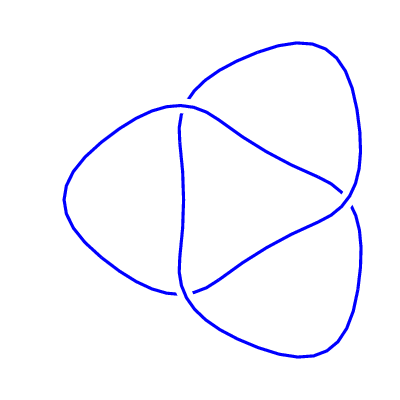
\includegraphics[width=\textwidth]{knotpics/3_1.png}
        \caption{A trefoil knot}
    \end{subfigure}
    \hspace{1cm}
    \begin{subfigure}[b]{0.25\textwidth}
        \centering
        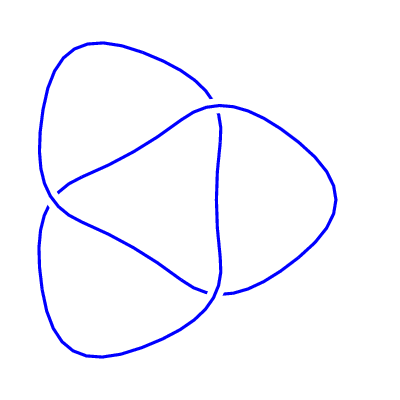
\includegraphics[width=\textwidth]{knotpics/3_1mirror.png}
        \caption{Another trefoil knot}
    \end{subfigure}
    \hspace{1cm}
    \begin{subfigure}[b]{0.25\textwidth}
        \centering
        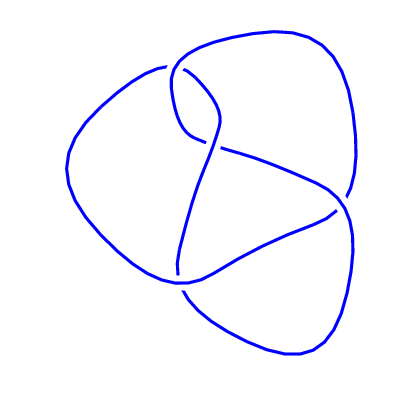
\includegraphics[width=\textwidth]{knotpics/4_1.png}
        \caption{A Figure Eight Knot}
    \end{subfigure}
    \caption{Several Interesting Knots with Few Crossings}
\end{figure}

Notice that in each of these we have represented the crossings by visually breaking the display of the strand that goes underneath. 
Look closely, the strand that goes over continues unbroken, but the strand that goes under stops and then restarts on the other side of the overstrand.
We don't really break the string!
This is a concession we have to make so that our drawing contains the vital information.



\begin{task}
Use your string to make both versions of the trefoil above. 
We want to know if they are really the same knot (they have the same name).
Try to find a way to rearrange the one string so that it becomes the other string.
That is, make the crossings look the same.
\end{task}

The \emph{unknot} is our standard ordinary circle.
It has this funny name in knot theory because we want to keep it around as a knot, but it is not knotted.
Yeah, unknot is easier to say.

\begin{task}
Try to use your string to show that the figure eight knot is essentially the same as the unknot.
\end{task}

The kind of physical twisting and rearranging you did with your strings while working on those tasks is an example of the kind of topological equivalence relevant to problems in knot theory. The technical term for this kind of sameness is \emph{ambient isotopy}. (If that feels uncomfortable, look up the words ambient and isotope.)

Now we have enough terms to state the 
\begin{quote}
\textbf{Fundamental Problem of Knot Theory}: Find a reasonable method to decide when two knots are equivalent under ambient isotopy.
\end{quote}

This problem is very hard.
Small parts of it have been handled, but sadly, it is still unsolved in general.

To give you stronger sense of the difficulty, consider the following pair of knots. These two knots gave mathematicians some trouble.

\begin{figure}[h]
    \centering
    \begin{subfigure}[b]{0.4\textwidth}
        \centering
        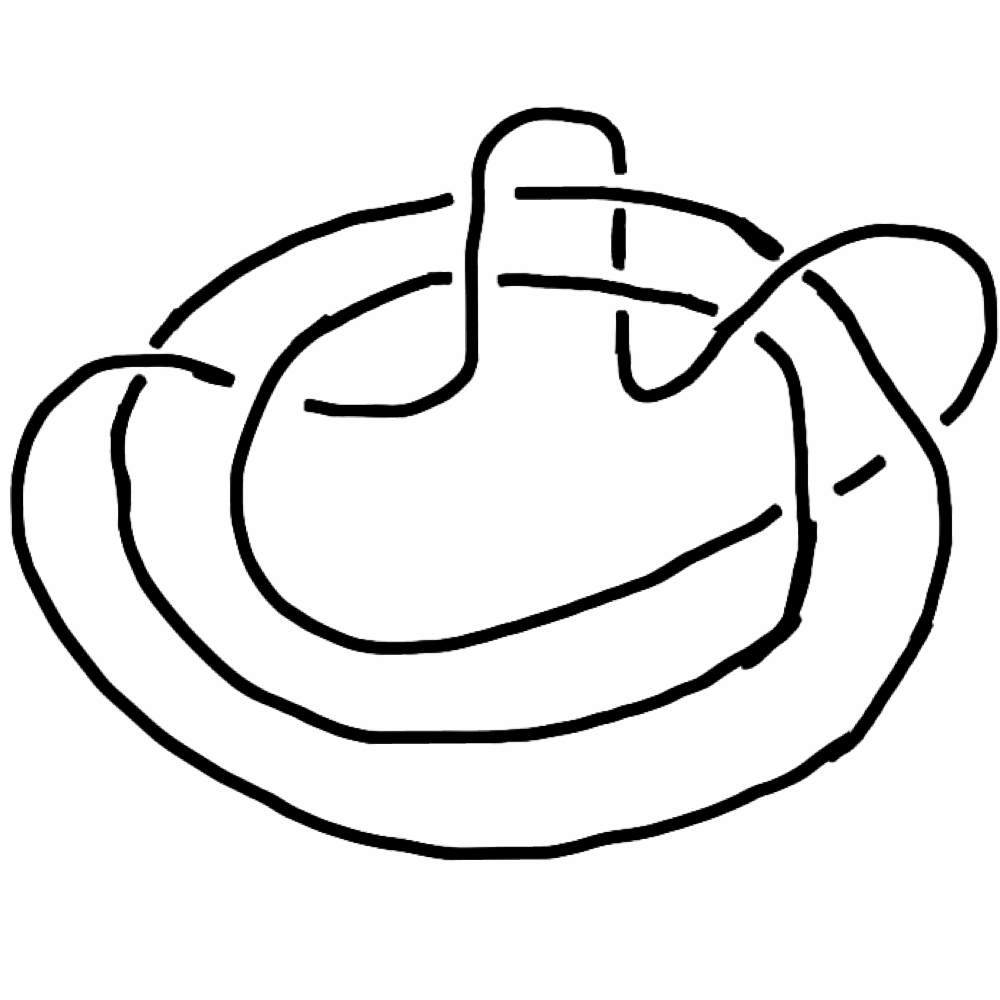
\includegraphics[width=\textwidth]{knotpics/perko1.png}
        \caption{Mystery Knot Number One}
    \end{subfigure}
    \hspace{1cm}
    \begin{subfigure}[b]{0.4\textwidth}
        \centering
        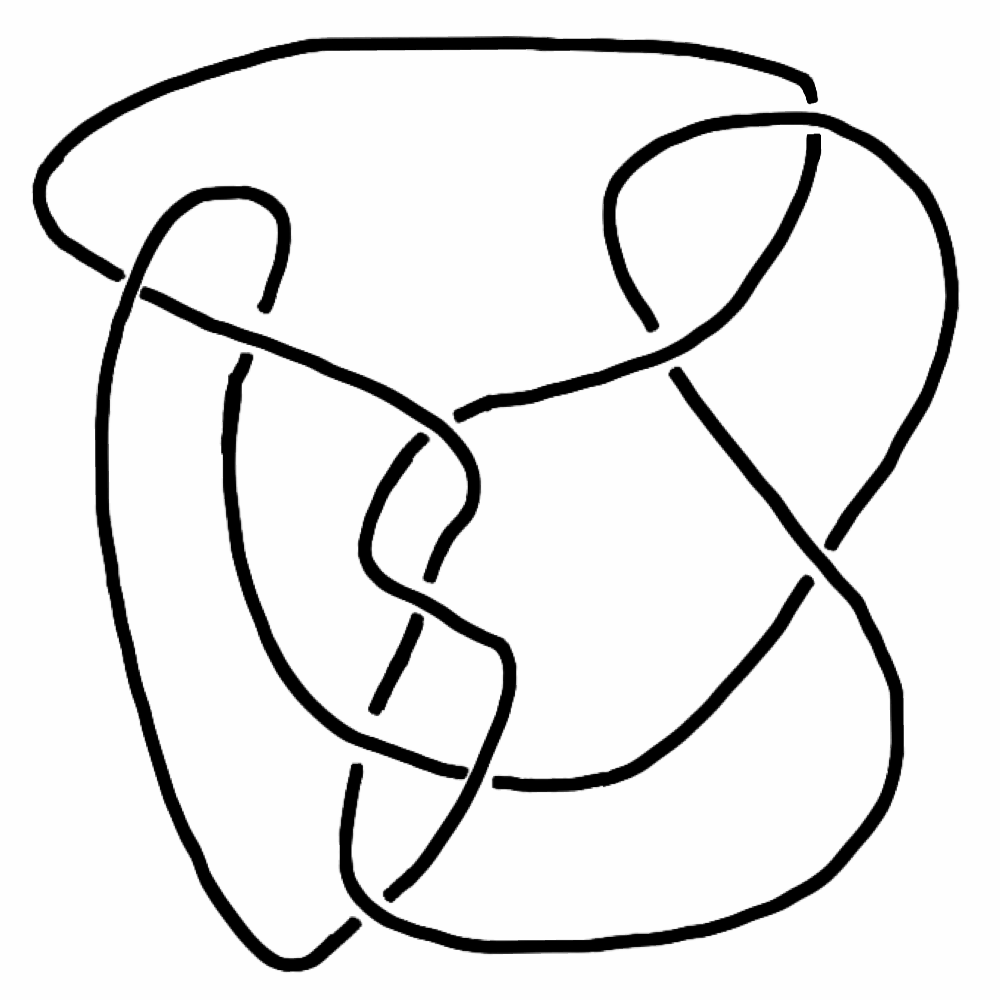
\includegraphics[width=\textwidth]{knotpics/perko2.png}
        \caption{Mystery Knot Number Two}
    \end{subfigure}
    \caption{A Pair of Naughty Knots}
\end{figure}

\begin{challenge}
Decide if these two knots are equivalent under ambient isotopy.
Or, to state it differently, but not really change the meaning: decide whether or not these two drawings are just different planar projections of the same knot.
\end{challenge}


\begin{thebibliography}{9}

\bibitem{Adams}
	Colin C. Adams,
	\emph{The Knot Book},
	American Mathematical Society, 
	2004.

\bibitem{ArtOfMath:knots}
	Philip K. Hotchkiss, with Volker Ecke, Julian F. Fleron, and Christine von~Renesse,
	\emph{Knot Theory},
	available online from \url{http://www.artofmathematics.org/}, 
	accessed August 15, 2013.

\bibitem{knotinfo}
	J. C. Cha and C. Livingston, 
	KnotInfo: Table of Knot Invariants, 
	\url{http://www.indiana.edu/~knotinfo}, 
	accessed: September 6, 2013.

\end{thebibliography}

\end{document}
%sagemathcloud={"zoom_width":100}